\chapter{Upload-Tool}\label{upload}
\section{Einsatzplaner}\label{upload:client}
Dieses Tool gibt ihnen die Möglichkeit die Listenansicht des Einsatzplans als PDF-Datei auf einen Webserver hochzuladen.
Dies kann manuell oder automatisch bei jedem Speichern geschehen.
Zur Konfiguration befindet sich im Datei-Menü ein Punkt "`Eigenschaften"'.
Durch diesen öffnet sich der Abschnitt in Abbildungn~\ref{fig:uploadtool}.
\begin{figure}[!h]
  \centering
	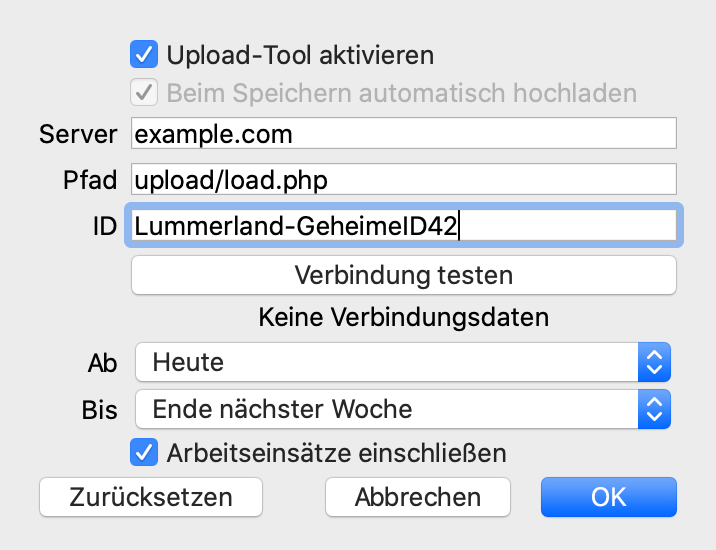
\includegraphics[width=0.5\textwidth]{img/eigenschaften_upload}
	\caption{Des Fenster der Dateieigenschaften}
	\label{fig:uploadtool}
\end{figure}
\begin{itemize}
  \item
  Mit dem ersten Haken wird das Tool aktiviert.
  \item
  Der zweite dient dazu einzustellen, ob die Datei automatisch hochgeladen wird, wenn die lokale Datei gespeichert wird.
  Diese Funktion ist nur verfügbar, wenn sie in den Programmeinstellungen aktiviert wurde (siehe Kapitel~\ref{einstellungen}.
  \item
  Unter Server, Pfad und ID geben Sie die Daten an, die Ihnen von Ihrem Webmaster mitgeteilt wurden.
  \neu{Bei Server ist das Protokoll mit anzugeben, sofern es sich nicht um \texttt{https} handelt, also \texttt{http} verwendet wird.}
  \item
  Mit dem Knopf können Sie testen, ob die Eingaben korrekt sind und eine Verbindung zum Server aufgebaut werden kann.
  Dabei werden keine Daten der Aktivitäten übermittelt.
\end{itemize}
Die drei letzten Einstellungen werden benötigt, wenn die Listenansicht automatisch hochgeladen werden soll.
Sie können einstellen, in welchem Zeitraum die Aktivitäten liegen müssen, damit Sie eingeschlossen werden.
Ebenso können Sie auswählen, ob Arbeitseinsätze auch ausgegeben werden sollen.

\hinweis{Beim Verwenden der Export-Funktion aus Kapitel~\ref{export} können Sie Beschränkungen festlegen, die unabhängig von diesen Einstellungen sind.}



\section{Server-Tool}\label{upload:server}
Zur Installation des Tools auf einem Server benötigen Sie eine nicht veraltete Version von PHP.
Die benötigten Dateien können von der Webseite des Programs (siehe Kapitel~\ref{sonstiges}) heruntergeladen werden.

Das Tool besteht aus der Konfigurationsdatei \texttt{config.php} und dem eigentlichen Programm \texttt{load.php}.
Der Name der Datei \texttt{load.php} kann an die eigenen Bedürfnisse angepasst werden.
Der Name der Konfigurationsdatei darf allerdings nicht verändert werden.
Ebenso müssen beide Dateien im gleichen Ordner liegen.

Die Konfiguration ist in der Datei \texttt{config.php} beschrieben.
